\documentclass[aspectratio=169]{beamer}

\usepackage[spanish,es-nodecimaldot]{babel}
\usepackage[utf8]{inputenc}
\usepackage[T1]{fontenc}
\usepackage{graphicx}
\usepackage{booktabs}
\usepackage{xcolor}
\usepackage{hyperref}
\usepackage{tikz}
\usepackage{amsmath}

\usetheme{Madrid}
\setbeamertemplate{navigation symbols}{}
\setbeamertemplate{footline}[frame number]

\title{Implementación de una red neuronal desde cero}
\subtitle{Problema XOR}
\author{Gianfranco Giannoni}
\institute{Herramientas para Ciencias de Datos\\
Docente: Michael Miranda\\
Universidad Tecnológica Metropolitana}
\date{11 de noviembre de 2026}

\begin{document}

\begin{frame}
\titlepage

\begin{tikzpicture}[remember picture,overlay]
\node[
    anchor=north west,
    xshift=1.1cm,
    yshift=-0.1cm
] at (current page.north west) {
    
\includegraphics[width=1.9cm]{logo_utem.png}
};
\end{tikzpicture}

\end{frame}

\begin{frame}{Objetivo y problema}
\begin{itemize}
    \item Implementar una red neuronal sin frameworks de deep learning.
    \item Utilizar Python y NumPy para las operaciones numéricas.
    \item Entrenar el modelo para resolver el problema XOR.
\end{itemize}
\vspace{0.3cm}
\begin{block}{¿Qué hace XOR?}
Entrega 1 cuando las entradas son distintas y 0 cuando son iguales.
\[
(0,0)\to 0,\quad (0,1)\to 1,\quad
(1,0)\to 1,\quad (1,1)\to 0.
\]
\end{block}
\end{frame}

\begin{frame}{Arquitectura de la red}
\centering
\begin{tikzpicture}[x=1cm,y=1cm, every node/.style={font=\small}]
    \foreach \y in {1.5,0.5} {
        \draw[fill=blue!15] (0,\y) circle (0.22);
    }
    \foreach \y in {2.1,1.1,0.1,-0.9} {
        \draw[fill=green!15] (3,\y) circle (0.22);
    }
    \draw[fill=orange!20] (6,0.6) circle (0.22);
    \foreach \a in {1.5,0.5} {
        \foreach \b in {2.1,1.1,0.1,-0.9} {
            \draw[gray] (0.23,\a) -- (2.77,\b);
        }
    }
    \foreach \b in {2.1,1.1,0.1,-0.9} {
        \draw[gray] (3.23,\b) -- (5.77,0.6);
    }
    \node[below] at (0,-1.25) {Entrada: 2};
    \node[below] at (3,-1.25) {Oculta: 4 (ReLU)};
    \node[below] at (6,-1.25) {Salida: 1 (Sigmoid)};
\end{tikzpicture}
\vspace{0.3cm}
\begin{block}{Arquitectura 2--4--1}
Dos entradas, una capa oculta de cuatro neuronas y una salida probabilística.
\end{block}
\end{frame}

\begin{frame}{Propagación hacia adelante}
La red calcula una predicción a partir de sus entradas y parámetros:
\[
Z_1=XW_1+b_1,\qquad A_1=\operatorname{ReLU}(Z_1)
\]
\[
Z_2=A_1W_2+b_2,\qquad \hat{Y}=\sigma(Z_2)
\]
\begin{itemize}
    \item $W$: pesos que multiplican las entradas.
    \item $b$: sesgos que desplazan la activación.
    \item ReLU: $\max(0,z)$.
    \item Sigmoid: transforma la salida a un valor entre 0 y 1.
\end{itemize}
\end{frame}

\begin{frame}{Pérdida y retropropagación}
\begin{block}{Binary Cross-Entropy}
Compara la probabilidad predicha con la etiqueta correcta:
\[
L=-\frac{1}{m}\sum_i
[y_i\log(\hat y_i)+(1-y_i)\log(1-\hat y_i)].
\]
\end{block}
\begin{itemize}
    \item La retropropagación calcula los gradientes de pesos y sesgos.
    \item En la salida, al combinar Sigmoid y BCE:
    \[
    dZ_2=\hat{Y}-Y.
    \]
    \item Los gradientes indican cómo cambia la pérdida al modificar cada parámetro.
\end{itemize}
\end{frame}

\begin{frame}{Aprendizaje: descenso del gradiente}
Los parámetros se actualizan en dirección opuesta al gradiente:
\[
\theta_{\text{nuevo}}=\theta_{\text{anterior}}-\alpha\nabla_\theta L
\]
\begin{itemize}
    \item $\alpha=0.1$: tasa de aprendizaje.
    \item 20\,000 épocas de entrenamiento.
    \item Se utilizan los cuatro ejemplos en cada actualización (full-batch).
\end{itemize}
\begin{block}{Idea central}
La red ajusta sus pesos y sesgos para reducir la pérdida y mejorar sus predicciones.
\end{block}
\end{frame}

\begin{frame}{Resultados}
\small
\begin{table}
\centering
\begin{tabular}{cc|c|c}
\toprule
Entrada & & Probabilidad & Clase predicha\\
$x_1$ & $x_2$ & $\hat y$ & \\
\midrule
0 & 0 & 0.0025 & 0\\
0 & 1 & 0.9997 & 1\\
1 & 0 & 0.9998 & 1\\
1 & 1 & 0.0002 & 0\\
\bottomrule
\end{tabular}
\end{table}
\begin{center}
\IfFileExists{training_loss.png}{
    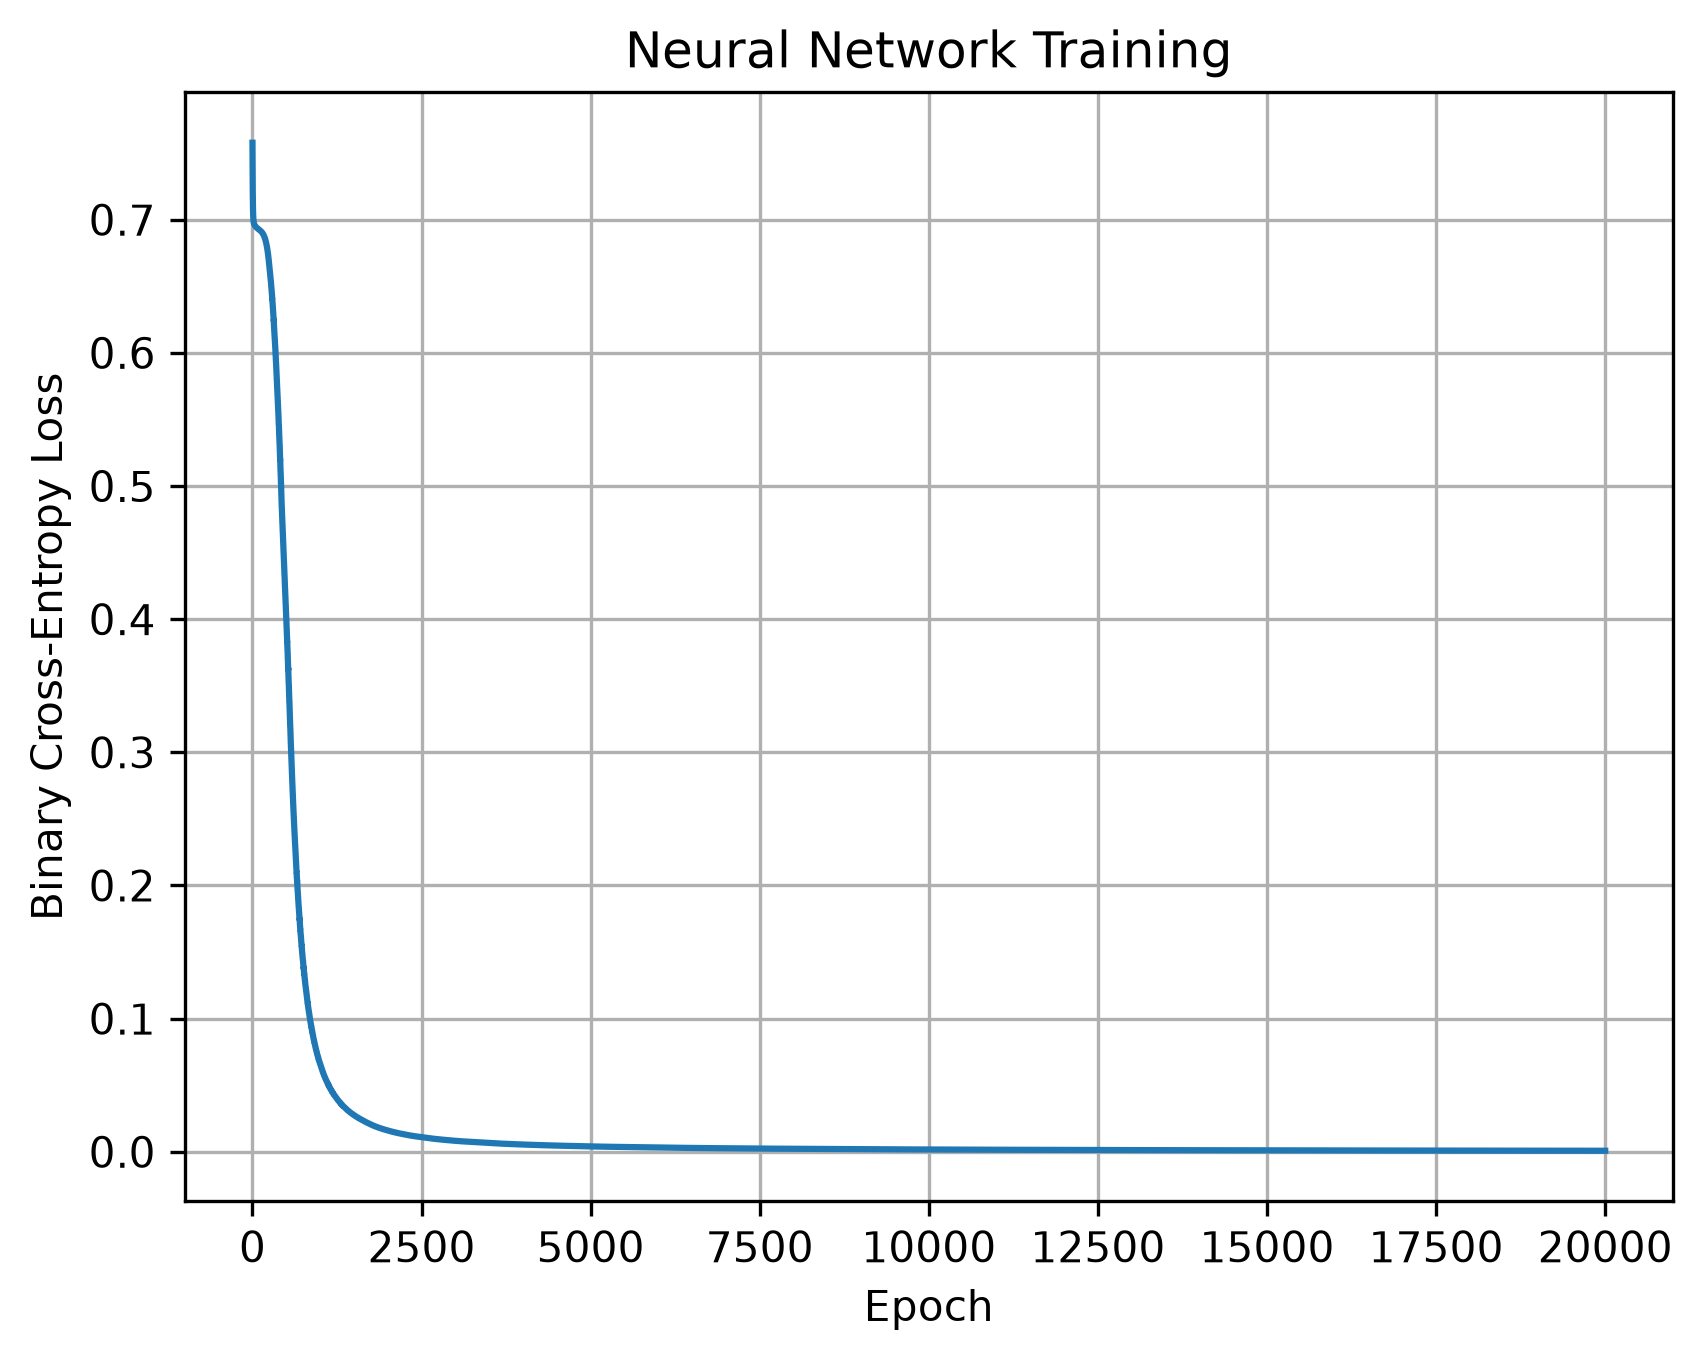
\includegraphics[width=0.68\textwidth,height=0.42\textheight,keepaspectratio]{training_loss.png}
}{
    \fbox{\parbox{0.68\textwidth}{\centering
    Gráfico pendiente: colocar \texttt{training\_loss.png} junto al archivo .tex.}}
}
\end{center}
\end{frame}

\begin{frame}{Conclusiones y limitaciones}
\begin{itemize}
    \item Se implementaron manualmente los pasos principales del aprendizaje de una red neuronal.
    \item La red 2--4--1 clasificó correctamente los cuatro casos XOR de entrenamiento.
    \item La capa oculta permite resolver este problema no linealmente separable.
    \item El conjunto es muy pequeño y no se evaluó con datos independientes.
\end{itemize}
\begin{block}{Conclusión}
El experimento demuestra el funcionamiento básico de una red neuronal entrenada mediante retropropagación y descenso del gradiente.
\end{block}
\end{frame}

\end{document}
